%!TEX program = xelatex
\documentclass[11pt,punct,twoside]{ctexart}
\usepackage{titling}
\usepackage[a4paper, left=3cm, right=2cm, top=3cm, bottom=2.5cm]{geometry}
\usepackage{fancyhdr, graphicx, xpatch, layout}
\usepackage{booktabs}
\usepackage{amsmath}
\usepackage{pdfpages}
\usepackage{float}
%\usepackage{cite}
\usepackage{enumitem}
\usepackage{titlesec}
\usepackage{titletoc}
\usepackage{tabularx}
\usepackage{chngcntr}
\usepackage{listings}
\usepackage{cleveref}
\usepackage{subfigure}
\usepackage[titles,subfigure]{tocloft}
\usepackage[labelsep=space]{caption}
\usepackage[numbers,super,square,comma,sort,compress]{natbib}
\usepackage{lmodern}
\usepackage{indentfirst}
\usepackage{xtab,booktabs}
\usepackage[version=4]{mhchem}
\usepackage{array}
\usepackage{fontspec}
\usepackage{caption}
\usepackage{xeCJK}
\usepackage{color}
\usepackage{longtable}
\usepackage{ctex}
%\usepackage{longtabu}
\usepackage{tabu}
\usepackage{makecell}
\usepackage{amssymb}
%\usepackage{showframe}

% 微分算子
\newcommand*{\dif}{\mathop{}\!\mathrm{d}}

% 参考文献行间距
\setlength{\bibsep}{-1pt}
%设置字体
\setmainfont{Times New Roman} % set all eng font
\songti%正文宋体
\zihao{-4}%正文小四号
\ctexset{section={format+={\mdseries\zihao{3}\heiti},aftername = \hspace{0.5em}}}%章标题 三号黑体
\ctexset{subsection={format+={\mdseries\zihao{-4}\heiti},aftername = \hspace{0.5em}}}%节标题 小四号黑体
\ctexset{subsubsection={format+={\mdseries\zihao{-4}\heiti},aftername = \hspace{0.5em}}}%级标题 小四号黑体  

%宋体伪粗体
\setCJKfamilyfont{zhsong}[AutoFakeBold = {2.17}]{SimSun}
\renewcommand*{\songti}{\CJKfamily{zhsong}}
%设置间距
\renewcommand{\baselinestretch}{1.62}
%\linespread{1.5}
\titlespacing{\section}{0bp}{0.5em}{0.5em}
\titlespacing{\subsection}{0bp}{0.5em}{0.5em}
\titlespacing{\subsubsection}{0bp}{0.5em}{0.5em}
%\setlength{\parskip}{0.5\baselineskip}
% 图表公式每章重新编号
\counterwithin{table}{section}
\counterwithin{figure}{section}
\counterwithin{equation}{section}

%表标题与内容间距
\setlength{\abovecaptionskip}{0.1cm}
%列表样式
\setlist[enumerate,1]{label=(\arabic*), wide, labelsep=0.5em, itemsep=0ex, topsep=0pt, partopsep=0pt, parsep=0pt}
\setlist[enumerate,2]{label=(\alph*) , wide, labelsep=0.5em, itemsep=0ex, topsep=0pt, partopsep=0pt, parsep=0pt,itemindent=5em}

%正文代码块lstlisting样式
\def\inline{\lstinline[basicstyle=\ttfamily,breaklines=true]}
\lstset{
	basicstyle=\ttfamily\zihao{5},
	xleftmargin=2em,
	%xrightmargin=2em,
    breaklines=true,
    frame={tb},
    belowcaptionskip=0.6em,
    framerule=1.5pt
}

%引用样式
\renewcommand{\lstlistingname}{代码清单}
\crefname{listing}{代码清单}{代码清单}
\crefname{table}{表}{表}
\Crefname{table}{表}{表}
\crefname{figure}{图}{图}
\Crefname{figure}{图}{图}

%自定义命令
\newcommand{\scite}[1]{\textsuperscript{\cite{#1}}} %cite样式
\DeclareCaptionFormat{myformat}{\zihao{5}\selectfont#1#2#3}
\captionsetup{format=myformat}
\captionsetup{labelsep=quad}%图表号与图表名之间空两格

%------------------文档开始------------------
\begin{document}
\pagestyle{empty}
\begin{titlepage}
	\begin{figure}[t]
		\centering
		
\includegraphics[width=0.92\textwidth]{images/cover.png}
	\vspace{-2.5em}
	\end{figure}
	
	\begin{center}
		\quad \\
		\quad \\
		\heiti \zihao{1} 《医疗数据处理实践》课程设计报告
		\vskip 0.5em
		\heiti \zihao{2} 泰坦尼克号幸存者数据分析及基于神经网络填充缺失值的预测模型
	\end{center}
	\vskip 1em
	
	\makeatletter
	
	\newcommand\dlmu[2][8em]{\underline{\hb@xt@ #1{\hss#2\hss}}}
	\makeatother	
	\begin{center}
		\zihao{-3}
		\heiti
		\renewcommand\arraystretch{0.72} 
		\setlength\extrarowheight{5mm} 
		\begin{tabular}[b]{b{-0.5em}b{4em}b{0.25em}b{16em}<{\centering}}
			%\cline{4-4}
			&\makebox[4em][s]{学\ \ \ \ \ \ \ \ 院}  &\ 	& 数\ 学\ 与\ 统\ 计\ 学\ 院 \\
			\cline{4-4}
			&\makebox[4em][s]{专\ \ \ \ \ \ \ \ 业}	&\ 	&数\ 据\ 科\ 学\ 与\ 大\ 数\ 据\ 技\ 术     \\
			\cline{4-4}
			&\makebox[4em][s]{班级序号}	&\ 	&\bf{200221}   \\
			\cline{4-4}
			&\makebox[4em][s]{学\ \ \ \ \ \ \ \ 号}	&\ 	&\bf{202015140}   \\
			\cline{4-4}
			&\makebox[4em][s]{姓\ \ \ \ \ \ \ \ 名}	&\ 	&周\ 华   \\ 
			\cline{4-4}
			&\makebox[4em][s]{指导教师}	&\ 	&王\  子\ 健\ 、\ 张\  建\ 波\ \\
			\cline{4-4}
			&\makebox[4em][s]{开始日期}	&\ 	&2022\  年\ 5\ 月\  28\ 日\ \\
			\cline{4-4}
			&\makebox[4em][s]{结束日期}	&\ 	&2022\  年\ 7\ 月\  6\ 日\ \\
			\cline{4-4}
		\end{tabular}
	\end{center}



		\vskip 1em
		\centering
\end{titlepage}
\clearpage
%\include{sections/statement}

%页眉页脚
\pagestyle{fancy}
%\setlength{\voffset}{3pt}
\lhead{}
\chead{\zihao{4}\heiti 概率论与数理统计(含随机过程)结课论文~~~~~~~~~~~~~~~~~~~~~~~~~~~~~~~~~~~~~~~~~~~~~~~~ 
\includegraphics[scale=0.15]{images/logo.png}}%\bfseries 不用加粗


\rhead{}
\lfoot{}
\cfoot{\zihao{5}\thepage}
\rfoot{}

\setlength{\voffset}{-10mm}                        
\setlength{\topmargin}{0mm}
\setlength{\headheight}{6mm}
\setlength{\headsep}{9mm}
\setlength{\footskip}{7.5mm}
\pagenumbering{Roman} %目录页码为罗马数字
\setcounter{page}{1}%页码重新计数

%正文代码块章节编号
\counterwithin{lstlisting}{section}

\section*{\zihao{-3}\heiti 泰坦尼克号幸存者数据分析及基于神经网络填充缺失值的预测模型}
\section*{\zihao{3}\heiti 摘\ \ \ \ \ \ \ \ 要}

泰坦尼克号是英国白星航运公司20世纪10年代建设的一搜豪华游艇。其排水量达到了惊人的4.6万吨,是当时世界上体积最大,最豪华的客运轮船。但正是这艘号称“永不沉没”的泰坦尼克号,在1912年从英国驶往美国时,在大西洋与冰山相撞并沉没!

根据英国贸易委员会公布的数据显示,在灾难发生时,泰坦尼克号共搭载2224人,其中710人生还,1514人不幸罹难,其中乘客约有1317人,共498人幸存;男性船员约有885人,共192人幸存;女性船员23人,共20人幸存。

本文通过数据分析与机器学习算法,对泰坦尼克号数据进行数据预处理,数据可视化,特征工程,模型调参,模型优化,有效提取了泰坦尼克号数据中的信息,并对幸存者建立了预测模型,模型准确率高达85.86\%。

\textbf{第一步}:首先进行导包,读取数据,然后查看数据基本信息,并对每个属性的数据进行剖析。\textbf{第二步}:对多个属性之间的关系进行分析,探索与可视化,得出幸存率主要与性别,年龄,船舱有关的结论。\textbf{第三步}:首先对无用信息、非数值型数据、缺失数据进行处理,然后训练神经网络模型并对Age数据进行预测填充。\textbf{第四步}:进行模型的训练与验证,模型调参与模型融合。
\par
 
 
 \par
%空一行

\noindent \zihao{-4}{\heiti 关键词:}\textbf{泰坦尼克号};\textbf{特征工程};\textbf{参数优化};\textbf{数据分析};\textbf{神经网络}

\clearpage


%\section*{\zihao{-3}\bfseries Research on Microstructure and Mechanical Properties of Mg/Al Composite Sheet during Rolling Process}

%\hfill Author: xxxx

%\hfill Tutor: xxxx

%\section*{\zihao{3}\bfseries Abstract}

%As a green material in the 21st century, magnesium alloys have the advantages of low density, high specific strength, excellent thermal conductivity, good damping, shock absorption and impact resistance. However, the low yield strength, high notch sensitivity and poor corrosion resistance of magnesium alloys greatly limit the large-scale industrial application of them. Al/Mg/Al composite sheets have high specific strength and corrosion resistance of magnesium alloys with the advantages of good plasticity, toughness and corrosion resistance of aluminum and its alloys. It has broad application prospects in automotive, aerospace and other fields. In this paper, Al/Mg/Al composite sheets were prepared by composite rolling based on AZ31B magnesium alloy and 1060 pure aluminium sheets. The effects of process parameters on the microstructure and mechanical properties of the composite sheets were revealed.
%	\\
	%空一行
%	\\
%	\zihao{-4}{\bfseries Key words:\ }AZ31B magnesium alloy; Composite rolling; Microstructure; Mechanical property; Intermetallic compounds

%\clearpage





%目录样式
% \renewcommand{\cftdot}{\ensuremath{\ast}}
\titlecontents{section}
              [1em]
              {}%
              {\contentslabel{1em}}%
              {}%
              {\titlerule*[0.32pc]{$\cdot$}\contentspage}
\titlecontents{subsection}
              [2.7em]
              {}%
              {\contentslabel{1.7em}}%
              {}%
              {\titlerule*[0.32pc]{$\cdot$}\contentspage}
\titlecontents{subsubsection}
              [5.5em]
              {}%
              {\contentslabel{2.5em}}%
              {}%
              {\titlerule*[0.32pc]{$\cdot$}\contentspage}
\renewcommand{\cftsecleader}{\cftdotfill{\cftdotsep}}
\newcommand\mydot[1]{\scalebox{#1}{.}}
\renewcommand\cftdot{\mydot{0.8}}
\renewcommand\cftdotsep{1}

\CTEXoptions[contentsname={\zihao{3}目\ \ \ \ \ \ \ \ 录}]
\renewcommand{\cftsecfont}{\heiti\zihao{-4}} %设置section条目的字体
\renewcommand{\cftsecpagefont}{\normalfont}
\renewcommand{\cftsubsecfont}{\songti\zihao{-4}} %设置subsection条目的字体
\rhead{}
\tableofcontents
\cleardoublepage
\pagenumbering{arabic} %正文页码为阿拉伯数字
\section{绪论}
回归,指研究一组随机变量$(y_1 ,y_2 ,\dots,y_i)$和另一组$(x_1,x_2,\dots,x_k)$变量之间关系的统计分析方法,又称多重回归分析。通常$y_1,y_2,\dots,y_i$是因变量,$x_1,x_2,\dots,x_k$是自变量。常见的回归算法包括最小二乘法回归,机器学习回归,KNN回归,神经网络回归等。

在回归问题中,对于某些离群值或者异常值,单个回归算法会产生较大误差。集成算法是一类构建多个学习器,通过一定策略结合来提高准确率,降低误差的模型。常见的集成算法分为Bagging、Boosting、Stacking三大类。本文主要使用了Bagging算法。

\subsection{回归算法}
\subsubsection{最小二乘法回归}
给定$n$个属性描述的自变量$\textbf{x}=(x_1,x_2,$\dots$,x_n)$,其中$x_i$为\textbf{x}在第$i$个元素上的取值。线性回归试图学得一个通过该属性的线性组合来进行预测的函数,即

\begin{equation}
f(\textbf{x})=w_1x_1+w_2x_2+\dots+w_nx_n+b, \label{1}
\end{equation}


一般用向量形式写成
\begin{equation}
f(\textbf{x})=\textbf{w}^T\textbf{x}+b,\label{2}
\end{equation}

其中$\textbf{w}=(x_1,x_2,$\dots$,x_n)$,$\textbf{w}$和$b$确定后,模型也得以确定。

给定数据集$D={((\textbf{x}_1,y_1),(\textbf{x}_2,y_2),\dots,(\textbf{x}_n,y_n)}$,其中$\textbf{x}_i=(x_{i1},x_{i2},\dots,x_{im}),y_i \in \mathbb{R}$.线性模型试图学得

\begin{equation}
f(\textbf{x}_i)=\textbf{w}^T\textbf{x}_i+b,~~~~~~~~s.t. ~~~~~~~~f(\textbf{x}_i)\approx y_i .\label{3}
\end{equation}
为了方便,我们令
 $$\mathop{w}\limits^{\^{}}=(\textbf{w},b) ,$$
 
 $$\textbf{x}=\begin{pmatrix}
 x_{11}&  x_{12}&  \dots&  x_{1d}& 1\\
 x_{21}&  x_{22}&  \dots&  x_{2d}& 1\\
 \vdots&  \vdots& \ddots  &  \vdots& \vdots\\
 x_{m1}&  x_{m2}&  \dots&  x_{md}& 1
 \end{pmatrix}=\begin{pmatrix}
 x_{1}^T& 1\\
 x_{2}^T& 1\\
 \vdots& \vdots\\
 x_{m}^T& 1
 \end{pmatrix},$$
 
 $$\textbf{y}=(y_1,y_2,\dots,y_m),$$
 其中,$\textbf{x}$是一个$m \times (d+1)$ 的矩阵,每行前$d$个元素对应集合$D$中的$d$个属性值。
 
 为了实现 \ref{3} ,我们使用均方误差来衡量$f(x_i)$与$y_i$之间的差别,以便确定最合适的$\textbf{w}$和$b$:
 \begin{equation}
E(f,D)=\frac{1}{m}\sum_{i=1}^m(f(x_i)-y_i)^2.\label{4}
 \end{equation}

 线性回归的任务转化为
 
 \begin{equation}
 \mathop{w}\limits^{\^{}}^*=arg_{\mathop{w}\limits^{\^{}}}min(\textbf{y}-\textbf{x}\mathop{w}\limits^{\^{}})^T(\textbf{y-x}\mathop{w}\limits^{\^{}}).
 \label{5}
 \end{equation}
 
令$E_{\mathop{w}\limits^{\^{}}}=(\textbf{y}-\textbf{x}\mathop{w}\limits^{\^{}})^T(\textbf{y-x}\mathop{w}\limits^{\^{}})$,对$\mathop{w}\limits^{\^{}}$求导得到
\begin{equation}
\frac{\partial E_{\mathop{w}\limits^{\^{}}}}{\partial \mathop{w}\limits^{\^{}}}=2\textbf{x}^T(\textbf{x}\mathop{w}\limits^{\^{}}-\textbf{y}).
\label{6}
\end{equation}

令\ref{6}等于零可以求得$\mathop{w}\limits^{\^{}}$最优解的闭式解。特殊地,当集合域D中只有一个属性时,可以求得
\begin{equation}
w=\frac{\sum\limits_{i=1}^my_i(x_i-\mathop{x}\limits^{-})}{\sum\limits_{i=1}^mx_i^2-\frac{1}{m}(\sum\limits_{i=1}^mx_i)^2},
\label{7}
\end{equation}

\begin{equation}
b=\frac{1}{m}\sum\limits_{i=1}^m(y_i-wx_i),
\label{8}
\end{equation}
其中$\mathop{x}\limits^{-}=\frac{1}{m}\sum\limits_{i=1}^mx_i$为$x$的均值.

现在对一个给定的数据点集用最小二乘法准则拟合$y=Ax^n$形式的曲线,n为固定数,研究模型$f(x)=ax^n$的最小二乘估计,应用该准则要求极小化$$s=\sum_{i=1}^m[y_i-f(x_i)]^2=\sum_{i=1}^m[y_i-ax_i^n]^2$$.最优化的必要条件是$\frac{dS}{da}=-2\sum_{i=1}^mx_i^n[y_i-ax_i^n]=0$,从方程可以解出a,得$$a=\frac{\sum x_i^ny_i}{\sum x_i^{2n}}$$
 






\subsubsection{机器学习回归}


在1.1.1中为了实现\ref{3},我们用均方误差\ref{4}来衡量拟合的曲线与实际数据的误差.当我们使\ref{4}取得最小值时,也就确定了最优解.神经网络使用梯度下降算法确定最优解.为了求出\ref{5},神经网络模型的计算步骤如下:



\clearpage


\begin{algorithm}[h]
	\caption{机器学习回归问题}
	\label{alg:4}
	\begin{algorithmic}[1]
		\STATE 随机初始化一组值$w_0$\
		\STATE 求解$\frac{\partial E_{\mathop{w}\limits^{\^{}}}}{\partial \mathop{w}\limits^{\^{}}}=2\textbf{x}^T(\textbf{x}\mathop{w}\limits^{\^{}}-\textbf{y})$\
		\STATE $w_1=w_0-\alpha \frac{\partial E_{\mathop{w}\limits^{\^{}}}}{\partial \mathop{w}\limits^{\^{}}}$,其中$\alpha$为常数,也称学习速率.
		\STATE $w_0=w_1$,重复3,直到$w_1<10^{-6}$
		\STATE 输出结果$w_1$
	\end{algorithmic}
\end{algorithm}





其中,特别地,当集合域D中只有一个属性时:
\begin{algorithm}[h]
	\caption{只有一个属性时机器学习解决回归问题}
	\label{alg:4}
	\begin{algorithmic}[1]
		\STATE 随机初始化一组值$w_0,b_0$\
		\STATE 求解$\frac{\partial E_{\mathop{w}\limits^{\^{}}}}{\partial \mathop{w}\limits^{\^{}}}$,$\frac{\partial E_{\mathop{w}\limits^{\^{}}}}{\partial \mathop{b}}$
		
		
		
		\STATE $w_1=w_0-\alpha \frac{\partial E_{\mathop{w}\limits^{\^{}}}}{\partial \mathop{w}\limits^{\^{}}}$,$b_1=b_0-\alpha \frac{\partial E_{\mathop{w}\limits^{\^{}}}}{\partial \mathop{b}\limits^{\^{}}}$其中$\alpha$为常数,也称学习速率.
		\STATE $w_0=w_1$,$b_0=b_1$,重复3,直到$w_1<10^{-6}$
		\STATE 输出结果$w_1,w_0$
	\end{algorithmic}
\end{algorithm}

机器学习能够解决的不仅只有线性回归问题,当知道目标函数后,即可使用剃度下降法求得目标函数的极值,从而求解各种回归问题。


\subsubsection{KNN回归}
KNN算法不仅可以用来聚类,还可以用来回归。KNN是一个简单的算法。简单的说就是取x距离最近的K个点,求它们的平均值作为预测值。
如图\ref{1}是一个K=3时用KNN回归的一个例子,KNN算法选取了最近的3个样本并取它们的平均值作为预测值。

\begin{figure}[h]
	\centering
	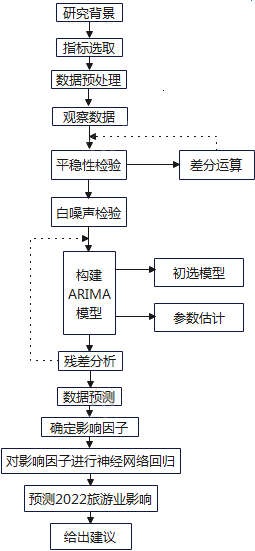
\includegraphics[scale=0.5,angle=0]{images/1.png}
	\caption{K=3时KNN回归的一个例子}
	\label{1}
\end{figure}


使用KNN回归的算法流程图如下:

\begin{document}
	% 例1
	\begin{algorithm}[h]
		\caption{KNN回归}
		\label{alg:Framwork}
		\begin{algorithmic}[1] %这个1 表示每一行都显示数字
			\REQUIRE ~~\\ %算法的输入参数:Input
			N个训练样本的集合  $A[n]$;\\
			人为设定的近邻个数$k$;\\
			给定的需要的预测的变量$x$:\\
			\ENSURE ~~\\ %算法的输出:Output
			预测的值$y$;
			\STATE 选择$A[1]$至$A[k]$作为$x$的初始近邻;
			\STATE 计算初始近邻与测试样本x间的欧氏距离$d(x, A[i]), i=1,2,...k$;
			\STATE 按$d(x, A[i])$从小到大排序;
			\STATE 计算最远样本与$x$间的距离$D$,即$max \{ d(x, A[j]) | j=1,2...k \} $;
			\STATE 
			
			 $for(i=k+1; i<n+1; i++)$ \{ 
			 
			 ~~~~~~~~~~~~~计算$A[i]$与$x$间的距离$d(x, A[i])$;
			  
			 ~~~~~~~~~~~~~$if (d(x, A[i]) < D )$
			 
			  ~~~~~~~~~~~~~~~~~~~~~~~~~~\{ 
			  
			  ~~~~~~~~~~~~~~~~~~~~~~~~~~用$A[i]$代替最远样本;  
			  
			  ~~~~~~~~~~~~~~~~~~~~~~~~~~ \}
			 
			 ~~~~~~~~~~~~~按照d(x, A[i])从小到大排序;
			 
			 ~~~~~~~~~~~~~计算最远样本与x间的距离D,即$max\{d(x, A[j]) | j=1,...i\}$;
			 
			 ~~~~~~~~~~~~~~~~~~~~~~~~~~~~~~~~~~~~~~~~~~~~~~~~~~~~\}
			
			\STATE 计算$y=\frac{1}{k} \sum_{i=1}^kd_i$
			\RETURN $y$; %算法的返回值
		\end{algorithmic}
	\end{algorithm}

\subsubsection{神经网络回归}
神经网络(Artificial Neural Networks,简写为ANNs)也简称为神经网络(NNs)或称作连接模型(Connection Model),它是一种模仿动物神经网络行为特征,进行分布式并行信息处理的算法数学模型。

神经网络在理论上能够拟合任意函数,包括非线性函数,是当下最流行的数学建模方法之一。

1959年两个生物科学家发现青蛙的神经元接受多个输入,输入包括青蛙的多个器官的输入,只有单输入的和到达一个阈值,才会有输出(青蛙接受的刺激比较大时才会有反应。

\begin{figure}[h]
	\centering
	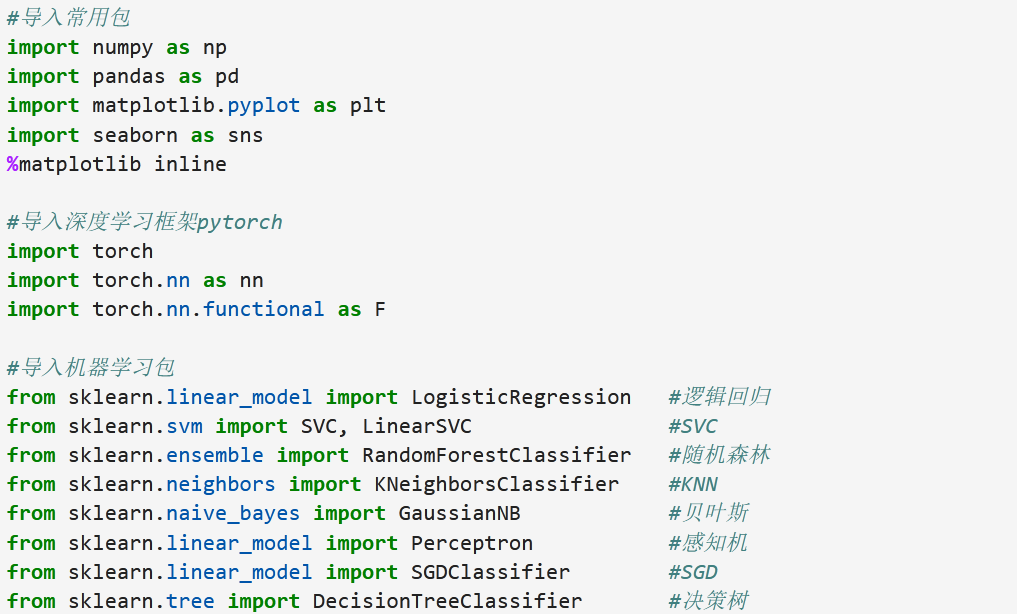
\includegraphics[scale=0.5,angle=0]{images/2.png}
	\caption{科学家研究青蛙的神经元原理}
	\label{2}
\end{figure}


于是计算机科学家仿照生物神经元的原理和结构,提出了感知器:
\begin{figure}[h]
	\centering
	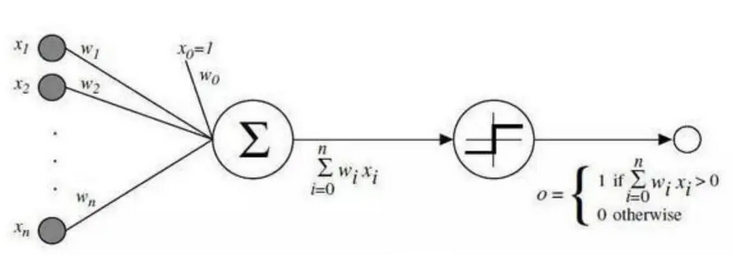
\includegraphics[scale=0.6,angle=0]{images/3.png}
	\caption{感知器}
	\label{3}
\end{figure}

经过不断完善和发展,形成了神经网络:
\begin{figure}[h]
	\centering
	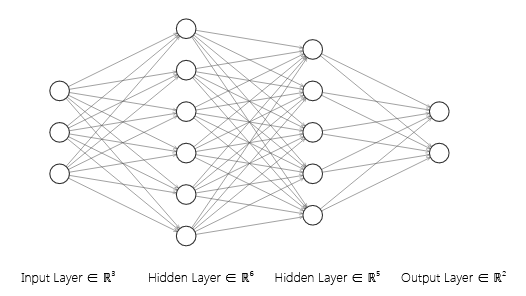
\includegraphics[scale=0.6,angle=0]{images/4.png}
	\caption{神经网络}
	\label{4}
\end{figure}

神经网络使用剃度下降法求解最优值,剃度下降法是一类求解函数最小值的计算机算法。假设希望求解目标函数 \textbf{$f(x)=f(x_1,\dots ,x_n)$}的最小值,可以从一个初始点 \textbf{$x^{(0)}=(x_1^{(0)},\dots,x_n^{(0)}})$}开始,基于学习率 \textbf{$\alpha > 0$} 构建一个迭代过程:

$$x_1^{i+1}=x_1^{i}+\alpha \frac{\partial f}{\partial x_1}(x^{(i)})$$
$$ \dots $$
$$x_1^{i+1}=x_1^{i}+\alpha \frac{\partial f}{\partial x_1}(x^{(i)})$$

其中$x^{(i)}=(x_1^{(i),\dots,x_n^{(n)}}),i>=0$,一旦达到收敛条件的话,迭代就结束了。图\ref{5}是用剃度下降法求解$y=x^2$的最小值的过程,其中的点代表每次迭代后的值。

\begin{figure}[h]
	\centering
	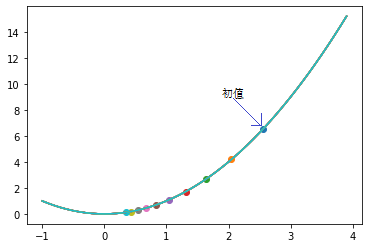
\includegraphics[scale=0.7,angle=0]{images/5.png}
	\caption{剃度下降法图解}
	\label{5}
\end{figure}
\subsection{Bagging算法}
Bagging算法 (英语:Bootstrap aggregating,引导聚集算法),又称装袋算法,是机器学习领域的一种团体学习算法。最初由Leo Breiman于1996年提出。Bagging算法可与其他分类、回归算法结合,提高其准确率、稳定性的同时,通过降低结果的方差,避免过拟合的发生。
Bagging算法描述如下所示.
\begin{figure}[h]
	\centering
	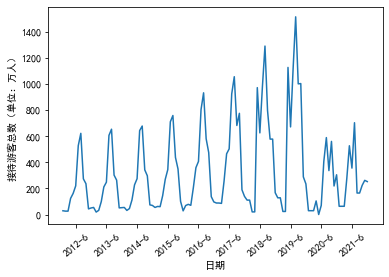
\includegraphics[scale=0.7,angle=0]{images/6.png}
	\caption{Bagging 算法}
	\label{6}
\end{figure}

Bagging算法就是将多个分类或者回归器同时训练,最后取平均值作为最终结果。其原理如图\ref{7}所示,其中输入为自变量,即需要输入的训练数据,$Function 1-4$为4个不同的分类器或者回归器,$y_i$为它们的输出结果,Bagging模型最终求其平均作为最终结果。

\begin{figure}[h]
	\centering
	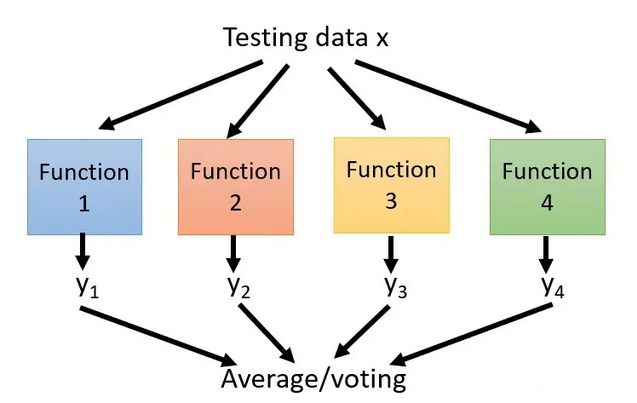
\includegraphics[scale=0.5,angle=0]{images/7.png}
	\caption{Bagging 算法图解}
	\label{7}
\end{figure}

\subsection{问题重述}
图 \ref{8} 是1898年到2012年明信片价格的变化,据此完成下列任务:
\begin{figure}[h]
	\centering
	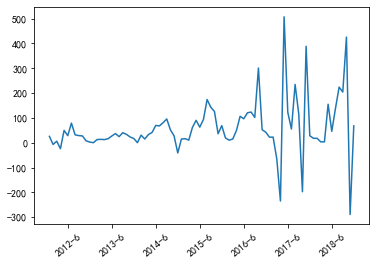
\includegraphics[scale=0.6,angle=0]{images/8.png}
	\caption{明信片价格变化}
	\label{8}
\end{figure}

\noindent (一)
\begin{itemize}
\item 使用最小二乘法建立曲线回归模型,预测2020年明信片的价格.

\item 使用机器学习的方法求解高阶多项式模型并预测2020年明信片的价格.

\item 建立KNN回归模型并预测2020年明信片的价格.

\item 建立神经网络回归模型并预测2020年明信片的价格.

\item 在上述四种模型的基础上建立Bagging算法模型并预测2020年明信片的价格.
\end{itemize}

\noindent (二)
\begin{itemize}
\item 比较以上5种回归模型的结果并选出最合适的模型,给出最终结果.
\end{itemize}

\section{问题求解}
\subsection{数据预处理}
我们将数据输入为csv文件,并对年份进行了处理:
$$x_i=x_i-x_1 +1$$以便更好的求解模型。


\subsection{最小二乘法拟合$ax^n$}
假定需要拟合的曲线为$y=ax^2$,研究$f(x)=ax^2$的最小二乘估计,应用准则要求极小化$$S=\sum_{i=1}^m[y_i-f(x_i)]^2=\sum_{i=1}^m[y_i-ax_i^2]^2$$最优化的必要条件是导数 $dS/da$等于0:$$\frac{dS}{da}=-2\sum_{i=1}^mx_i^n[y_i-ax_i^2]=0$$从方程中解出a,得$$a=\frac{\sum x_i^2y_i}{\sum x_i^4}=0.001981$$
因此,回归方程为$$y=0.001981 * x^2$$,当$x=2020-1898+1=123$时,$$y=29.97$$


\begin{figure}[h]
	\centering
	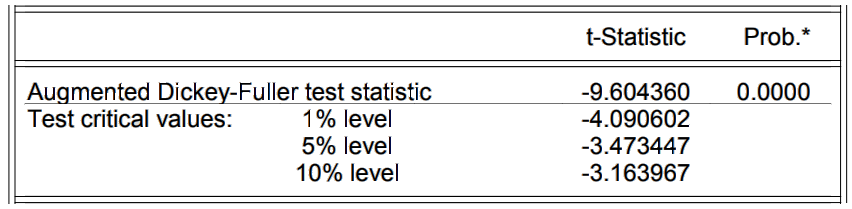
\includegraphics[scale=0.5,angle=0]{images/9.png}
	\caption{拟合结果}
	\label{9}
\end{figure}

\subsection{剃度下降法拟合高阶多项式模型}
假设需要拟合的曲线为$$y=a_0+a_1x+a_2x^2+\dots+a_{10}x^{10}$$

损失函数为$$loss=\sum(y(x_i)-y_i)^2$$


初始化一组解$$a_0=a_1=\dots=a_{10}=1$$
求解
\begin{equation}
grad_{a_j}=\frac{dloss}{da_j}=2 \sum(y(x_i)-y_i) \sum x_i^j
\end{equation}
求解
\begin{equation}
a_i=a_i - \alpha *grad_{a_i}
\end{equation}
,其中 $\alpha = 0.001,i=1,2,\dots,10.$迭代2.1与2.2,直到$|grad_{a_i}|$<=0.001.通过计算机程序可求得:

$y=- 1.639136814e-15*x^{10} + 1.059936718e-12*x^9 - 0.0000000002960388319*x^8 $

$+ 0.00000004652752046*x^7 - 0.000004472787601*x^6 + 0.0002650337924*x^5$ 

$- 0.00900509148*x^4 + 0.126851489*x^3 + 1.240266286*x^2 $

$- 47.08797047*x + 46.72959737.$


当$x=123$时,$y=13.78$

\begin{figure}[h]
	\centering
	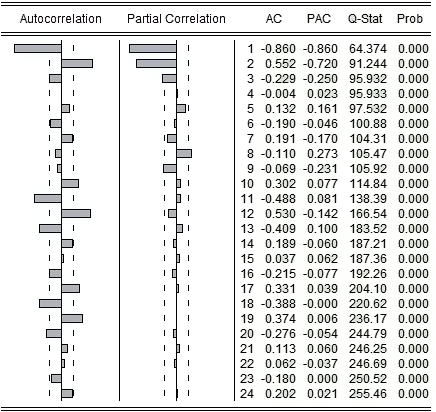
\includegraphics[scale=0.55,angle=0]{images/10.png}
	\caption{拟合结果}
	\label{10}
\end{figure}


\subsection{KNN回归}
我们使用KNN进行回归,得出以下结果:


\begin{figure}[H]
	\centering
	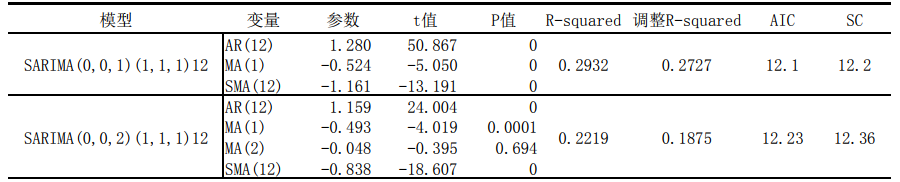
\includegraphics[scale=0.55,angle=0]{images/11.png}
	\caption{拟合结果}
	\label{11}
\end{figure}

当$x=123$时,$$y=29.67$$


\subsection{神经网络回归}
我们建立下面的神经网络,并进行训练.

\begin{figure}[H]
	\centering
	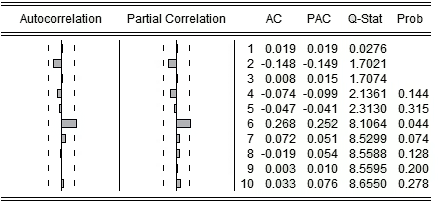
\includegraphics[scale=0.4,angle=0]{images/12.png}
	\caption{回归模型}
	\label{12}
\end{figure}

其中,学习速率 $\alpha=0.001$,最终拟合结果如图\ref{13}所示,当$x=123$时,$$y=34.00$$
\begin{figure}[h]
	\centering
	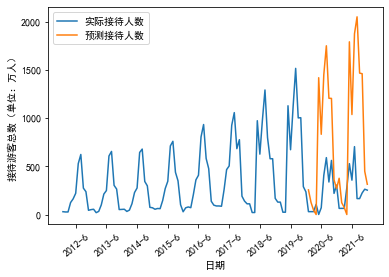
\includegraphics[scale=0.55,angle=0]{images/13.png}
	\caption{拟合结果}
	\label{13}
\end{figure}







\subsection{Bagging}
最后,我们使用Bagging算法对上面的四种结果取平均,其中,注意到,高阶多项式模型的误差比较大,因此Bagging算法选用其他三种回归算法。算法流程图如下。
\begin{figure}[h]
	\centering
	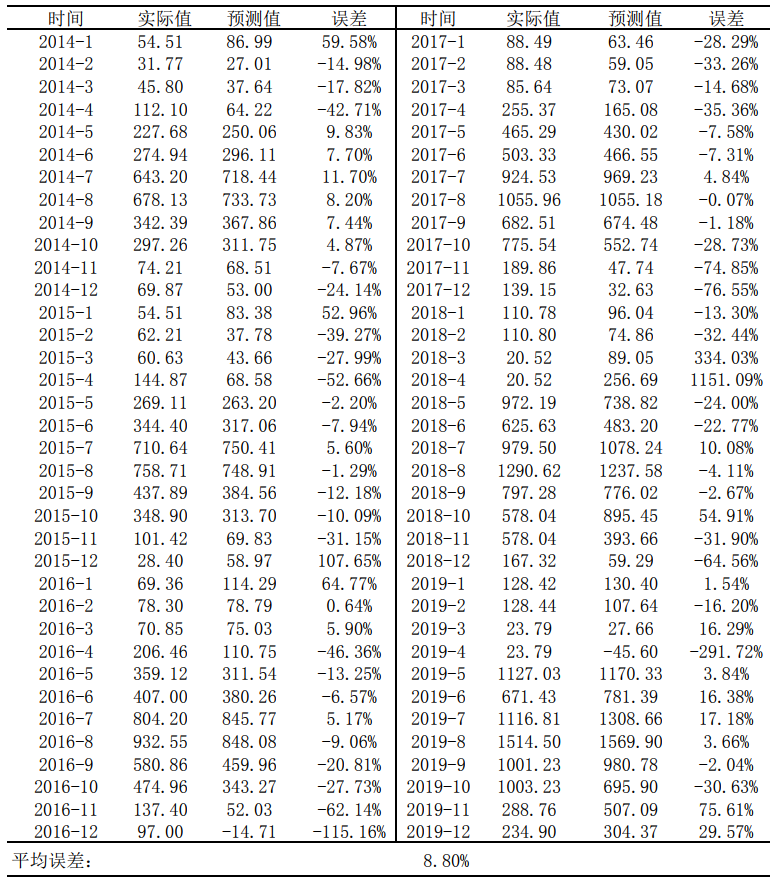
\includegraphics[scale=0.45,angle=0]{images/14.png}
	\caption{Bagging算法}
	\label{14}
\end{figure}

根据Bagging算法,可以求得$$y=\frac{1}{3}(34.00+29.67+29.97)=31.21$$


\section{模型比较}
\subsection{数据预处理}
为了能够更好的比较模型的准确度,我们从数据中抽取一半的数据用于建立模型,剩下的一半数据用于判断模型的准确度。数据分布如下:
\begin{figure}[h]
	\centering
	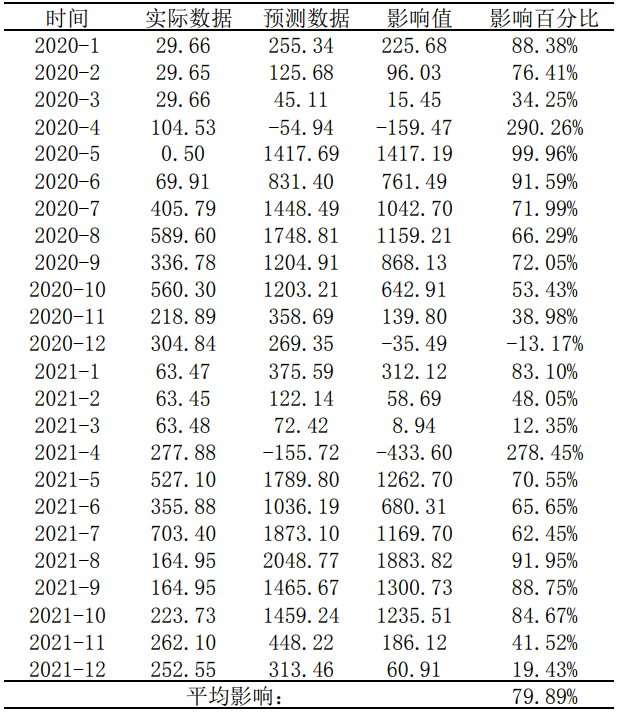
\includegraphics[scale=0.6,angle=0]{images/15.png}
	\caption{数据划分}
	\label{15}
\end{figure}


\subsection{最小二乘法回归}
假定需要拟合的曲线为$y=ax^2$,研究$f(x)=ax^2$的最小二乘估计,应用准则要求极小化$$S=\sum_{i=1}^m[y_i-f(x_i)]^2=\sum_{i=1}^m[y_i-ax_i^2]^2$$最优化的必要条件是导数 $dS/da$等于0:$$\frac{dS}{da}=-2\sum_{i=1}^mx_i^n[y_i-ax_i^2]=0$$从方程中解出a,得$$a=\frac{\sum x_i^2y_i}{\sum x_i^4}=0.001956$$
因此,回归方程为$$y=0.001981 * x^2$$.


\begin{figure}[h]
	\centering
	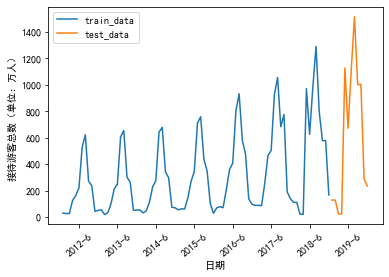
\includegraphics[scale=0.55,angle=0]{images/16.png}
	\caption{拟合结果}
	\label{16}
\end{figure}
测试数据的均方误差为
$$E=\frac{1}{m}\sum_{i=1}^m(f(x_i)-y_i)^2=4395.53.}$$


\subsection{剃度下降法拟合高阶多项式模型}
假设需要拟合的曲线为$$y=a_0+a_1x+a_2x^2+\dots+a_{10}x^{10}$$

损失函数为$$loss=\sum(y(x_i)-y_i)^2$$


初始化一组解$$a_0=a_1=\dots=a_{10}=1$$
求解
\begin{equation}
grad_{a_j}=\frac{dloss}{da_j}=2 \sum(y(x_i)-y_i) \sum x_i^j
\end{equation}
求解
\begin{equation}
a_i=a_i - \alpha *grad_{a_i}
\end{equation}
,其中 $\alpha = 0.001,i=1,2,\dots,10.$迭代2.1与2.2,直到$|grad_{a_i}|$<=0.001.通过计算机程序可求得:

$3.975590632e-13*x^10 - 0.0000000003290771782*x^9 $

$+ 0.0000001204184953*x^8 - 0.00002556825203*x^7 $

$+ 0.003471943435*x^6 - 0.3127761976*x^5 + 18.70628778*x^4 $

$- 717.4565232*x^3 + 16097.80278*x^2 - 165200.0207*x + 149802.2775$


\begin{figure}[h]
	\centering
	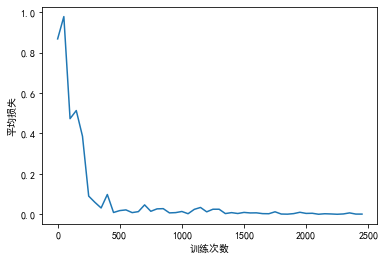
\includegraphics[scale=0.5,angle=0]{images/17.png}
	\caption{拟合结果}
	\label{17}
\end{figure}

测试数据的均方误差为
$$E=\frac{1}{m}\sum_{i=1}^m(f(x_i)-y_i)^2=177174.24.}$$



\subsection{KNN回归}
我们使用KNN进行回归,得出以下结果:


\begin{figure}[h]
	\centering
	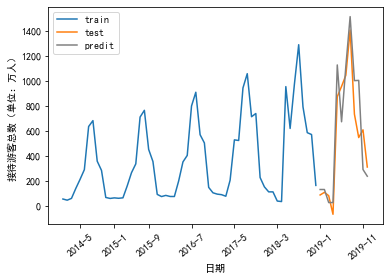
\includegraphics[scale=0.5,angle=0]{images/18.png}
	\caption{拟合结果}
	\label{18}
\end{figure}

测试数据的均方误差为
$$E=\frac{1}{m}\sum_{i=1}^m(f(x_i)-y_i)^2=25636.22.}$$


\subsection{神经网络回归}
我们采用第二节的神经网络2.4模型进行训练.
其中,学习速率 $\alpha=0.001$,最终拟合结果如图\ref{13}所示,当$x=123$时,$$y=34.00$$
\begin{figure}[h]
	\centering
	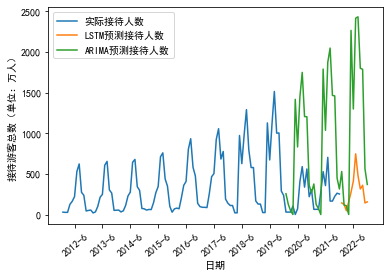
\includegraphics[scale=0.5,angle=0]{images/19.png}
	\caption{拟合结果}
	\label{19}
\end{figure}



测试数据的均方误差为
$$E=\frac{1}{m}\sum_{i=1}^m(f(x_i)-y_i)^2=31.2013.}$$





\subsection{Bagging}
最后,我们使用Bagging算法对上面的四种结果取平均,其中,注意到,高阶多项式模型的误差比较大,因此Bagging算法选用其他三种回归算法。

\begin{figure}[h]
	\centering
	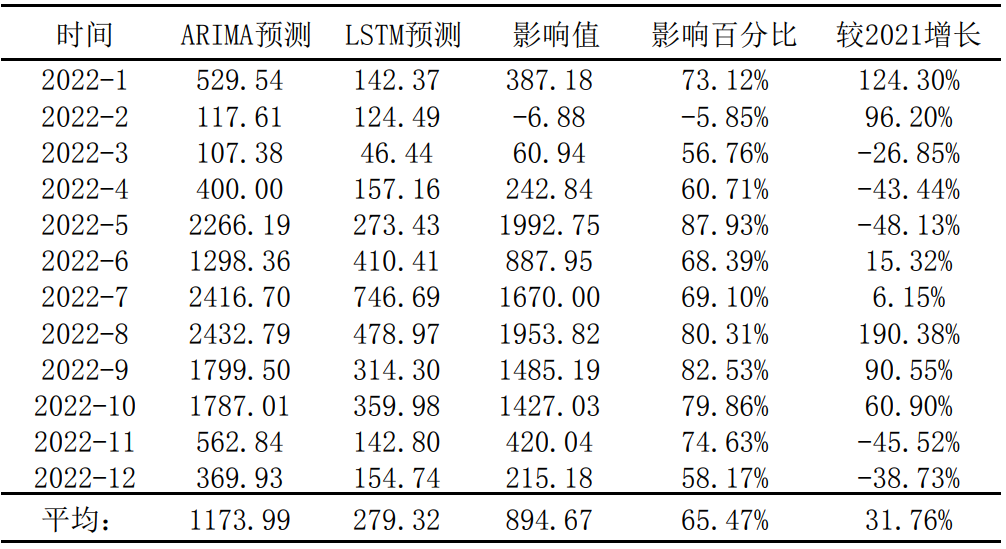
\includegraphics[scale=0.5,angle=0]{images/20.png}
	\caption{拟合结果}
	\label{20}
\end{figure}

测试数据的均方误差为:
$$E=\frac{1}{m}\sum_{i=1}^m(f(x_i)-y_i)^2=24614.14}$$

\subsection{最终结果}


\begin{table}[htbp]
	\centering
	\caption{不同回归方法的比较}
	
\begin{tabular}{|p{4.5cm}| p{3.5cm}| p{2.5cm}|}%会有5列,指定每列的居中形式,|表示每列中间有竖线分开
	\hline%每行之间由横线分开
	回归方法&2020年预测结果&均方差   \\%\\表示换行
	\hline
	最小二乘法曲线回归&29.97&2723090.92\\
	\hline
	高阶多项式回归&13.78&177174.24\\
	\hline
	KNN回归&29.67&25636.22\\
	\hline
	神经网络回归&34.00&31.2013\\
	\hline
	Bagging模型&31.21&24614.14\\
	\hline	
\end{tabular}
\end{table}	
\\

综上所述,选用神经网络回归效果最好,测试数据的均方误差为
$$E=31.2013.$$,2020年明信片价格预测结果为$$y=34.00$$


\section{总结}
从模型的结果来看,神经网络的拟合效果是最好的。其中KNN回归原理虽然简单,但是效果良好;而高阶多项式回归在数据集两侧的误差则特别大。Bagging模型的拟合效果虽然不如神经网络,但优于其他回归方法,具有提高准确率,降低过拟合的作用。





%\include{sections/Experimentalmaterials}
%\include{sections/Micro-organizationanalysis}
%\include{sections/Mechanicsperformanceanalysis}

%\include{sections/conclusion}
%\include{sections/thanks}

%\bibliographystyle{plain}
\bibliographystyle{unsrt}
\nocite{*}
\addcontentsline{toc}{section*}{参考文献}

\renewcommand\bibnumfmt[1]{\makebox[0.9cm][l]{[#1]}}
\setlength{\bibhang}{0em}


\begin{thebibliography}{99}
	\bibitem{book1}邓集贤,杨维权,司徒荣,邓永录.概率论与数理统计.下册(第四版).北京:高等教育出版社,2009.7
	
	\bibitem{art1}财务视角下新冠肺炎疫情对贵州工业发展影响的统计测度[C]//中国统计教育学会.2020年(第七届)全国大学生统计建模大赛优秀论文集.[出版者不详],2020:25.DOI:10.26914/c.cnkihy.2020.045581.
	
	\bibitem{art2}新冠肺炎疫情对青海省旅游业影响的统计研究——基于SARIMA模型[C]//中国统计教育学会.2020年(第七届)全国大学生统计建模大赛优秀论文集.[出版者不详],2020:16.DOI:10.26914/c.cnkihy.2020.045584.
	
	\bibitem{book2}周志华. 机器学习 [J]. 清华大学出版社, 2016, 8(28): 1–415.
	
	\bibitem{art3}[1]. 新冠疫情对海南旅游业影响的统计测度研究[C]//中国统计教育学会.2020年(第七届)全国大学生统计建模大赛优秀论文集.[出版者不详],2020:29.DOI:10.26914/c.cnkihy.2020.045597.
	
	\bibitem{book3}王燕.应用时间序列分析.中国大学出版社,2005.7
\end{thebibliography}	




%\include{sections/appendix}

\end{document}